\documentclass{beamer}
\usepackage[english,russian]{babel}
\usepackage[utf8]{inputenc}
\usepackage[T1,T2A]{fontenc}
% Стиль презентации
\usetheme{Warsaw}
\usecolortheme{dove}

%---------Формулы
\newcommand{\vF}{\mathbf{F}}
\newcommand{\ve}{\mathbf{e}}
\newcommand{\vk}{\mathbf{k}}
\newcommand{\vq}{\mathbf{q}}
\newcommand{\vp}{\mathbf{p}}
\newcommand{\va}{\mathbf{a}}
\newcommand{\vP}{\mathbf{P}}
\newcommand{\vK}{\mathbf{K}}
\newcommand{\vQ}{\mathbf{Q}}
\newcommand{\vA}{\mathbf{A}}
\newcommand{\vr}{\mathbf{r}}
\newcommand{\vR}{\mathbf{R}}

\newcommand{\vRR}{\boldsymbol{\mathcal{R}}}
\newcommand{\veps}{\boldsymbol{\varepsilon}}

\newcommand{\cA}{\mathcal{A}}
\newcommand{\cR}{\mathcal{R}}
\newcommand{\cM}{\mathcal{M}}
\newcommand{\cE}{\mathcal{E}}
\newcommand{\cJ}{\mathcal{J}}
\newcommand{\cT}{\mathcal{T}}
\newcommand{\cD}{\mathcal{D}}
%----------------

%---------Колонтитулы
\makeatletter
\defbeamertemplate*{headline}{my theme}{}
\defbeamertemplate*{footline}{my theme}{
	\leavevmode%
	\hbox{%
		\begin{beamercolorbox}[wd=.8\paperwidth,ht=2.25ex,dp=1ex,center]{title in head/foot}%
			\usebeamerfont{title in head/foot}\inserttitle
		\end{beamercolorbox}%
		\begin{beamercolorbox}[wd=.2\paperwidth,ht=2.25ex,dp=1ex,right]{date in head/foot}%
			\usebeamerfont{date in head/foot}\insertframenumber{} / \inserttotalframenumber\hspace*{2ex}
	\end{beamercolorbox}}%
}
\makeatother
%--------------------


\begin{document}
\title{Использование метода перевала в нестационарных задачах квантовой механики}  
\author{Махно А А}
\institute[ВГУ]{Воронежский государственный университет}
\date{}
% Создание заглавной страницы
\frame
{
	\titlepage 
	\small\centering{Руководитель Флегель А В}
} 


% Автоматическая генерация содержания
\frame{\frametitle{Содержание}\tableofcontents} 


\frame
{
	\frametitle{Постановка задачи}
	\section{Постановка задачи}
	В квантовой механике одноэлектронная математическая модель атома, подверженного воздействию лазерного импульса, описывается нестационарным уравнением Шредингера для электронной волновой функции
	$$
	\left[i\hbar\frac{\partial}{\partial t} + \frac{\hbar^2}{2 m} \nabla^2 - U(r) - V(\vr, t)\right]\Psi(\vr, t) = 0
	$$
}

\frame
{
	\frametitle{Постановка задачи}
	Волновая функция при $r \rightarrow \infty$
	\begin{equation}\label{A}
		\Psi(\vr, t) = -\frac{2\pi\hbar^2}{m k} \int_{-\infty}^{t} e^{-i\epsilon t'/\hbar} G(\vr, t;0, t')f(t')dt',
	\end{equation}
	где $G(\vr, t;\vr', t')$ - функция Грина, имеющая вид
	\begin{equation}\nonumber
	\label{Green}
	G(\vr,t;\vr',t') = -\theta(t-t')\frac{i}{\hbar}\left[\frac{m}{2\pi i\hbar(t-t')}\right]^{3/2}e^{iS(\vr,t;\vr',t')/\hbar},
	\end{equation}
	Граниченое условие при $r \rightarrow 0$
	\begin{equation}\label{B}
	\Psi(\vr, t) \sim \left(B(\epsilon) + \frac{1}{r}\right)f(t)e^{-i\epsilon t/\hbar}
	\end{equation}
}

\frame
{
	\frametitle{Постановка задачи}
	Переходя в атомную систему единиц $(|e| = m_e = \hbar = 1)$, и сшивая уравнения (\ref{A}) и (\ref{B}), получаем систему:
	\begin{eqnarray}\label{system}
		\sum_{n = -\infty}^{0}[B(\epsilon + n\omega) - i(2(\epsilon + n\omega))^{1/2}]f_ne^{-i n\omega t} = \nonumber\\
		= \sum_{m = -\infty}^{0} \cM(\epsilon + m\omega,t)f_me^{i m \omega t}, 
	\end{eqnarray}
	где для расчета образа фурье функции f $(f_i)$,  
	потребуется вычислять матричный элемент
	\begin{equation}\label{input}
		\cM(\epsilon, t) = \sqrt{\frac{1}{2\pi i}}\int_{0}^{\infty}\frac{e^{i\epsilon\tau}}{\tau^{3/2}}\left[e^{iS(t, t-\tau)} - 1\right].
	\end{equation}
}

\frame
{
	\frametitle{Метод перевала}
	\section{Метод перевала}
	Метод перевала применяется для оценки при больших значениях параметра $\lambda$ интегралов вида
	\begin{equation}\nonumber
	I(\lambda) = \int_{a}^{b}\phi(t)e^{\lambda f(t)}dt
	\end{equation}
	Преобразуя их к виду
	\begin{equation}\nonumber
	I(\lambda) \sim e^{\lambda f (z_0)}\sqrt{\frac{2\pi}{|f^{\prime \prime} (z_0)|}} \phi(z_0) e^{i \theta} \frac{1}{\sqrt{\lambda}},
	\end{equation}
	где $z_0$ - корни уравнения $f'(t) = 0$.
	
	В интеграле $\cM(\epsilon,t)$ роль большого параметра $\lambda$ играет величина:
	
	\begin{equation}\label{eq.lambda}
	\lambda = \frac{1}{2 \cT} \int_{-\cT/2}^{\cT/2} A^2(\tau) d\tau.
	\end{equation}
}

\frame
{
	\frametitle{Аналитическое ршение}
	\section{Аналитическое ршение}
	Итоговая формула, получанная методом перевала
	\begin{equation}
	\cM(\epsilon, t) \simeq \sum_{t_0}\frac{e^{i\widetilde{S}(t, t_0)} }{\sqrt{D} (t-t_0)^{3/2}},
	\end{equation}
	где $\widetilde{S} = \epsilon (t - t_0) + S(t, t_0)$,
	$$
	D = \alpha(t_0, t, t_0)\left[F(t_0) - \frac{1}{(t - t_0)^2} \int_{t_0}^{t}A(\tau)d\tau +  \frac{A(t_0)}{t-t_0} \right]
	$$
	и $t_0$ - корни уравнения $\alpha ^2 (t_0, t, t_0) = 2 \epsilon$.	
}

\frame
{
	\frametitle{Аналитическое решение}
	Рассмотрим вклад точки $t = t'$ в интеграл $\cM$
	
	\begin{center}
		\includegraphics{I_0}  
	\end{center}	
}

\frame
{
	\frametitle{Аналитическое решение}
	Решим уравнение $\alpha ^2 (t_0, t, t_0) = 2 \epsilon$ для $\epsilon \ge 0$.
	На рисунке изображена функция $\alpha (t', t, t')$, t = 0.
	
	\begin{center}
		\includegraphics{alpha-200}  
	\end{center}	
}


\frame
{
	\frametitle{Аналитическое решение}
	Аналогично, $\alpha (t', t, t')$ для случая t = 20.
	
	\begin{center}
		\includegraphics{alpha-2020}  
	\end{center}	
}

\frame
{	
	\frametitle{Численное решение}
	\section{Численное решение}
	Для получения точного численного решения использовалась библиотека GNU GSL, а также FFTW.
	Сравнивая вид преобразования Фурье с видом искомого интеграла $\cM$, получаем $(t = const)$, что если
	$$ 
	f(\tau) = \frac{1}{{\tau}^{3/2}}(e^{i S(t, t-\tau)} - 1)
	$$
	и
	$$
	\hat{f}(\xi) = \int_{0}^{\infty} e^{i \tau \xi} f(\tau) d\tau,
	$$
	то
	$$
	\cM(\epsilon,t)=\frac{1}{\sqrt{2\pi i}} \hat{f}(\epsilon).
	$$	
}

\frame
{
	\frametitle{Численное решение}	
	Значение $\epsilon$ может не совпасть с одной из частот преобразования, в таком случае используем линейное приближение.
	
	\begin{center}
		\includegraphics{fftw_compare_nofftw2}  
	\end{center}	
}

\frame
{
	\frametitle{Сравнение результатов}
	\section{Сравнение результатов}
	Решения седлового уравнения для различных параметров
	
	\begin{center}
		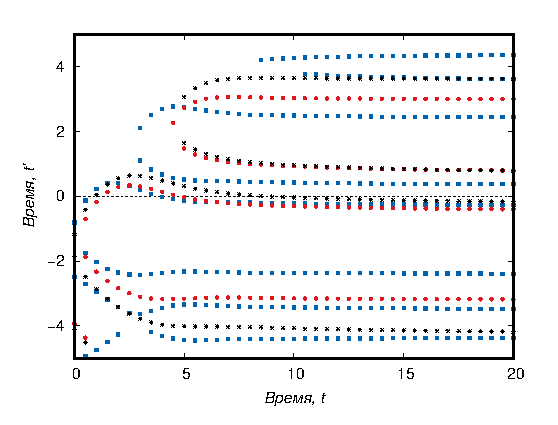
\includegraphics{roots2}  
	\end{center}	
}

\frame
{
	\frametitle{Сравнение результатов}
	Сравнение решений для параметров $\epsilon = 0.4$, $F_0 = 2$, $\omega = 0.8$
	
	\begin{center}
		\includegraphics{full1}  
	\end{center}	
}

\frame
{
	\frametitle{Сравнение результатов}
	Сравнение решений для параметров $\epsilon = 0.4$, $F_0 = 2$, $\omega = 0.8$ на отрезке $t = [20,70]$
	
	\begin{center}
		\includegraphics{end1}  
	\end{center}	
}

\frame
{
	\frametitle{Сравнение результатов}
	Сравнение решений для параметров $\epsilon = 0.35, F_0 = 2.2, \omega = 0.8$
	
	\begin{center}
		\includegraphics{full2}  
	\end{center}	
}

\frame
{
	\frametitle{Сравнение результатов}
	Сравнение решений для параметров $\epsilon = 0.35, F_0 = 2.2, \omega = 0.8$ на отрезке $t = [20,70]$
	
	\begin{center}
		\includegraphics{end2}  
	\end{center}	
}

\frame
{
	\frametitle{Сравнение результатов}
	Изменим параметр $F_0$ ($\epsilon = 0.35, F_0 = 1.6, \omega = 0.8$).
	
	\begin{center}
		\includegraphics{full3}  
	\end{center}	
}

\frame
{
	\frametitle{Сравнение результатов}
	Уменьшение параметра $F_0$ влечет за собой уменьшение величины $\lambda$, что ухудшает перевальную оценку
	
	\begin{center}
		\includegraphics{end3}  
	\end{center}	
}

% Создание заглавной страницы
\frame
{
	\titlepage 
	\small\centering{Руководитель Флегель А В}
} 

\frame
{
	\frametitle{Краткий список литературы}
	\begin{thebibliography}{}
		\bibitem{litlink1}  Араманович И.Г. Левин В.И. Уравнения математической физики. М.: Наука, 1969. 288 с.
		\bibitem{litlink2}  М.В. Федорюк. Метод перевала. М.: Главная редакция физико-математической литературы изд-ва «Наука», 1977. 368 с.
		\bibitem{other-link-name1}  Лаврентьев М.А Шабат Б.В. Методы теории функций комплексного переменного. М.: Главная редакция физико-математической литературы изд-ва «Наука», 1973. 736 с.
		\bibitem{other-link-name2}  Wong R. Asymptotic Approximations of Integrals. NY.: SIAM, 2001. 543 p.
	\end{thebibliography}
}
\end{document}
